\section{Billedanalyse}
Kamera api giver adgang til kamera, det kræver at brugeren aktivt selv tager billedet. Data er et billede eller en videosekvens.

\subsection{Autonom billed capture}
Da der formentlig skal tages et billede en gang om dagen for at have tilstrækkelig data skal patienten aktivt selv tage et billede, for eksempel hver morgen.
Det vurderes at være problematisk i forhold til at patienten kan ``snyde'' med sit humør.
Vi har derfor overvejet muligheden for at få telefonen til selv at tage billeder i baggrunden ved bestemte begivenheder, fx. når skærmen tændes eller patienten skriver en sms.
Det kan lade sig gøre ved at bruge ansigtgenkendelse.

\subsection{Ansigtsgenkendelse}
Android har indbygget funktioner til at finde ansigter i et billede. 
Vi kan der efterfølgende skrive kode der genkender ansigter fra hinanden, og vi kan på den måde sikre os at vi kun analyserer billeder af ejeren(se første link).

Se følgende links:
\begin{enumerate}
\item \url{https://github.com/yaylas/AndroidFaceRecognizer}

\item \url{http://bytefish.de/blog/face\_detection\_with\_android/}

\item \url{http://developer.android.com/guide/topics/media/camera.html#face-detection}
	
\end{enumerate}

\subsection{Pupil reaktion}
Vi forestiller os at vi kan lave en kort videosekvens hvor patienten bliver blitzet i perioden, for at analysere på pupillens reaktion til blitzen, se \cite{hoeks1993pupillary}.
Det er dog et problem at de fleste telefoner kun har blitz på bagsiden.

\subsection{Humør}

Et billede af en patient kan analyseres for at finde patientens humør. 
For at få en objektiv vurdering vurderes det at telefonen selv skal tage billeder i tilfældige tidsintervaller. 
Se \cite{kulkarni2009facial}
\begin{figure}
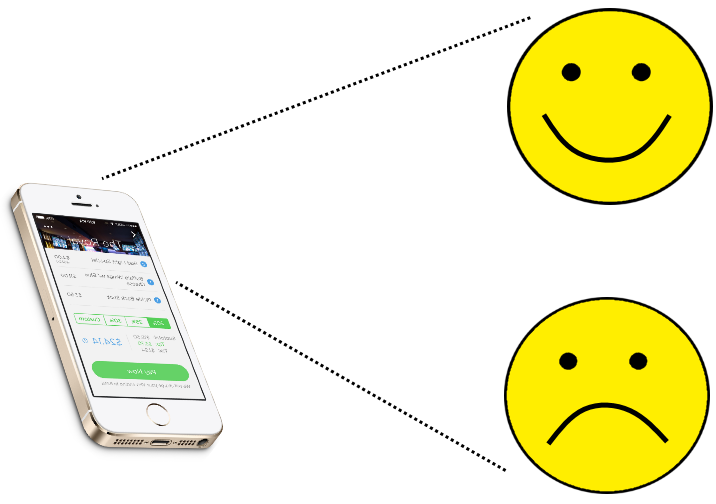
\includegraphics[width=\textwidth]{humoer}
\caption{En bruger er ved at bruge telefonen. Imens, uden at vedkommende ved det, tages der et billede vha. front kameraet. Det tjekkes at billedet er af telefonens ejer og derefter evalueres vedkommendes humør.}
\end{figure}